\documentclass[crop,tikz]{standalone}
\usetikzlibrary{backgrounds}
\colorlet{blue}{cyan}
\tikzset{
  inverted/.style = {
    color=white,
    background rectangle/.style={fill},
    show background rectangle
  }
}

\usetikzlibrary{angles}
\tikzset{>=latex}

\begin{document}
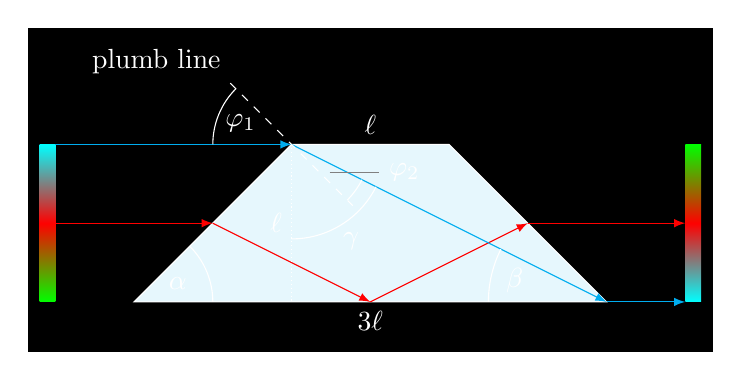
\begin{tikzpicture}[inverted,inverted]
  \pgfmathsetmacro{\length}{2};
  % 
  \draw[fill=cyan!10]
  ({-1.5*\length},0) coordinate (O)
  -- ++ ({3*\length},0) coordinate (A)
  -- ++ ({90+45}:{sqrt(2)*\length})
  -- ++ ({-\length},0) coordinate (B)
  -- cycle;
  \pic[draw,angle radius=1cm,pic text={$\alpha$}] {angle = A--O--B};
  % 
  \draw[->,red] ({-2*\length},{\length/2}) -- ++({\length},0) coordinate (Y1);
  \draw[->,red] (Y1) -- (0,0) coordinate (Y2);
  \draw[->,red] (Y2) -- ({\length},{\length/2}) coordinate (Y3);
  \draw[->,red] (Y3) -- ++({\length},0);
  % 
  \shade[top color=blue,bottom color=green,middle color=red] ({-2.1*\length},0) rectangle ++({0.1*\length},{\length});
  \shade[top color=green,bottom color=blue,middle color=red] ({ 2.0*\length},0) rectangle ++({0.1*\length},{\length});
  % 
  \node[above] at (0,{\length}) {$\ell$};
  \node[below] at (0,0) {$3\ell$};
  % Solution
  \draw[->,blue] ({-2*\length},{\length}) coordinate (U) -- ({-\length/2},{\length}) coordinate (X1);
  \draw[->,blue] (X1) -- ({1.5*\length},0) coordinate (X2);
  \draw[->,blue] (X2) -- ++({\length/2},0);
  % 
  \draw[densely dotted] (X1) -- node[left] {$\ell$} ({-\length/2},0) coordinate (F);
  \draw[dashed] (X1)++({90+45}:1.1) coordinate (L2) -- ++ (-45:2.2) coordinate (L) node[above left,pos=0] {plumb line};
  \pic[draw,angle radius=1cm,pic text={$\varphi_1$},angle eccentricity=0.7] {angle = L2--X1--U};
  \pic[draw,angle radius=1cm,pic text={\phantom{.}},pic text options={pin={[pin edge={gray,shorten <=-5pt}]0:{$\varphi_2$}}}] {angle = L--X1--A};
  \pic[draw,angle radius=1.5cm,pic text={$\beta$},angle eccentricity=0.8] {angle = X1--A--O};
  \pic[draw,angle radius=1.2cm,pic text={$\gamma$},angle eccentricity=1.2] {angle = F--X1--A};
\end{tikzpicture}
\end{document}
